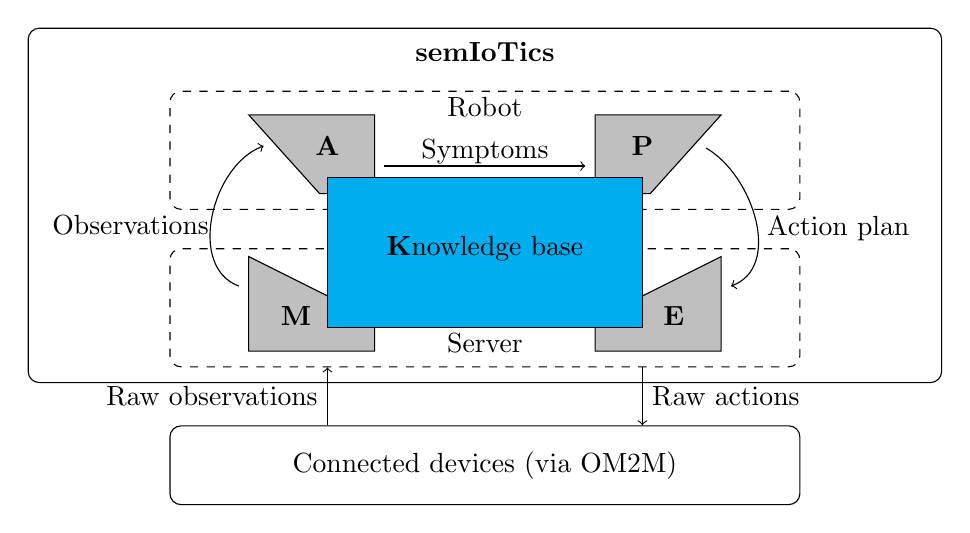
\begin{tikzpicture}

	% Connected devices
	\draw (0,0.75) node[draw, rectangle, rounded corners, minimum width=8cm, minimum height=1cm] (om2m) {} ;
	% SemIoTics
	\draw (0,2.75) node[draw, dashed, rectangle, rounded corners, minimum width=8cm, minimum height=1.5cm] (server) {} ;
	% Robots
	\draw (0,4.75) node[draw, dashed, rectangle, rounded corners, minimum width=8cm, minimum height=1.5cm] {} ;
	
	\draw (0,4.05) node[draw, rectangle, rounded corners, minimum width=11.6cm, minimum height=4.5cm] {} ;
	
	% M
	\draw[fill=lightgray] (-3, 2.2) -- node[pos=0.65] (M2A) {} (-3,3.4) -- (-1.4,2.6) -- (-1.4,2.2) -- cycle;
	% A
	\draw[fill=lightgray] (-3, 5.2) -- (-1.4,5.2)  -- node[pos=0.65] (A2P) {} (-1.4,4.2) -- (-2.1,4.2) -- node[pos=0.65] (AFM) {} cycle;
	% P
	\draw[fill=lightgray] (3, 5.2) -- (1.4, 5.2)  -- node[pos=0.65] (PFA) {} (1.4, 4.2) -- (2.1, 4.2) -- node[pos=0.65] (P2E) {} cycle;
	% E
	\draw[fill=lightgray] (3, 2.2) -- node[pos=0.65] (EFP) {} (3,3.4) -- (1.4,2.6) -- (1.4,2.2) -- cycle;
	% kb
	\draw[fill=cyan] (-2, 2.5) -- (2,2.5) -- (2,4.4) -- (-2,4.4) -- cycle;
	\draw[->] (M2A) to[out=160, in=200] node[pos=0.45, left, xshift=0.1cm] {Observations} (AFM);
	\draw[->] (A2P) -- node [above, yshift=-0.1cm] {Symptoms} (PFA);
	\draw[->] (P2E) to[out=330, in=20] node[pos=0.55, right] {Action plan} (EFP);
	\draw[->] ([xshift=-2cm]om2m.north) -- node[pos=0.5, left] {Raw observations} ([xshift=-2cm]server.south);
	\draw[<-] ([xshift=2cm]om2m.north) -- node[pos=0.5, right] {Raw actions} ([xshift=2cm]server.south);
	\draw (0,0.75) node {Connected devices (via OM2M)};
	\draw (0,2.3) node {Server};
	\draw (0,5.3) node {Robot};
	\draw (0, 6) node {\textbf{semIoTics}};
	\draw (-2.4,2.65) node {\textbf{M}};
	\draw (-2,4.8) node {\textbf{A}};
	\draw (2,4.8) node {\textbf{P}};
	\draw (2.4,2.65) node {\textbf{E}};
	\draw (0, 3.5) node {\textbf{K}nowledge base};
	
	
\end{tikzpicture}